\section{Prototipo vertinimas}

Šiame skyriuje pristatomas tyrimas, kurio metu vertinama įgyvendinto roboto URL adresų peržiūros ir Javascript atvaizdavimo greitaveika, taip pat atskirų sistemos komponentų apkrovos.

\subsection{Tyrimo aprašymas}

Tiriant saityno peržiūros roboto greitaveiką, mokslinėje literatūroje dažniausiai vertinamas peržiūrėtų URL adresų skaičius per laiko vienetą, taip pat iš viso surastų URL nuorodų skaičius \cite{HeritrixArchitecture}. Dėl to, šio tyrimo metu stebėti pasirinktos šios funkcinės prototipo greitaveikos charakteristikos:

\begin{enumerate}
    \item \textbf{Peržiūrėtų URL adresų skaičius}
    \item \textbf{Vidutiškai peržiūrėtų URL adresų / s}
    \item \textbf{Visų surastų URL adresų skaičius}
    \item \textbf{JS variklio pagalba atvaizduotų URL adresų skaičius}
    \item \textbf{JS variklio pagalba surastų URL adresų skaičius}
    \item \textbf{JS variklio pagalba surastų URL adresų dalis (proc.)}
\end{enumerate}

4,5,6 punktai pasirinkti dėl rašto darbo temos išskirtinumo tirti modernių saityno programų žvalgymo greitaveiką ir stebėti, ar reikšmingą surandamų URL adresų dalį sudaro adresai, rasti pasitelkiant JS atvaizdavimo variklio pagalbą.

\subsubsection{Vykdytos iteracijos}

Vykdytos 7 skirtingos iteracijos (kiekviena iteracija trunka lygiai 1 val.), kurių metu didintas lygiagrečiai veikiančių aktyvių peržiūros ir Javascript atvaizdavimo agentų skaičius tokia tvarka:

\begin{enumerate}
    \item \textbf{ 1 peržiūros agentas + 1 Javascript atvaizdavimo agentas}
    \item \textbf{2 peržiūros agentai + 1 Javascript atvaizdavimo agentas}
    \item \textbf{4 peržiūros agentai + 2 Javascript atvaizdavimo agentas}
    \item \textbf{8 peržiūros agentai + 4 Javascript atvaizdavimo agentas}
    \item \textbf{16 peržiūros agentų + 8 Javascript atvaizdavimo agentas}
    \item \textbf{32 peržiūros agentai + 16 Javascript atvaizdavimo agentas}
\end{enumerate}

Tokia seka tyrimui pasirinkta, nes ji buvo taikyta \cite{MercedCloudBasedWebCrawler} šaltinyje aprašyto debesų kompiuterijos technologijomis paremto saityno peržiūros roboto, kurio architektūros principais remiasi šio rašto darbo prototipas, tyrime. Dvigubai mažesnis Javascript  atvaizdavimo agentų skaičius pasirinktas tikintis, jog Javascript atvaizdavimo poreikis sudarys tik gana nedidelę dalį visų peržiūrėtų URL adresų.

\subsubsection{Roboto komponentų apkrovos}

\cite{MercedCloudBasedWebCrawler} moksliniame straipsnyje aprašytame peržiūros roboto tyrime stebėtos architektūroje naudojamų bendrų komponentų apkrovos (komponentų, į kuriuos kreipiasi kiekvienas peržiūros agentas). Stebėti „Azure Queue“ ir „Azure Table Storage“ komponentų vidutiniai uždelsimų laikai, priklausantys nuo tranzakcijų skaičiaus. Įgyvendinant šio rašto darbo prototipą, vietoje „Azure Queue“ pasirinkta „Service Bus Queues“ eilių infrastruktūros paslauga, kuri neturi vidutinio uždelsimo laiko vertinimo metrikos, dėl šios priežasties eilių mechanizmui stebėti pasirinkta ateinančių užklausų skaičiaus metriką per sekundę (angl. -- \textit{Incoming Requests per second}), taip pat atmestų užklausų kiekis (angl. -- \textit{Throttled Requests}). „Azure Service Bus Standard Tier“ planas, kuris naudojamas šio prototipo tyrime, apibrėžia maksimalų skiriamą kreditų kiekį per laiko vienetą, t.y. -- 1000 kreditų per sekundę \cite{ServiceBusThrottlingOverview}. Viršijus šį limitą, visos perviršiaus užklausos yra atmetamos, kol kreditai atstatomi. Ateinančių užklausų skaičius bus stebimas siekiant nustatyti, kada būtų artėjama prie šios ribos. Tyrimo metu stebimi komponentai ir jų metrikos:

\begin{itemize}
    \item \textbf{„Azure Service Bus Queue“ eilių infrastruktūra (agentų peržiūros eilės)} -- ateinančių užklausų skaičius per sekundę ir atmestų užklausų skaičius
    \item \textbf{„Azure Table Storage“ (URL adresų repozitorija) }-- tranzakcijų skaičius ir vidutinis uždelsimo laikas (taip pat, kaip stebėta \cite{MercedCloudBasedWebCrawler} aprašytame tyrime)
    \item \textbf{ SQL Agentų registras: DTU\footnote{DTU -- Data Transaction Unit: „Azure“ abstrakti metrika, skirta įvertinti duombazės resursų naudojimą} išnaudojimas, proc. } -- \cite{MercedCloudBasedWebCrawler} tyrime nenagrinėta, tačiau pasirinkta, nes šio prototipo realizacija stipriai priklauso nuo SQL duomenų bazės (automatinis peržiūros agentų išregistravimas remiantis paskutiniu aktyvumo laiku, saugomu agentų registro lentoje)
    \item \textbf{ Išeinantis tinklo srautas, GB (angl. -- \textit{egress traffic})} -- \cite{MercedCloudBasedWebCrawler} tyrime nenagrinėta, tačiau pasirinkta, nes svarbu įvertinti realius piniginius kaštus vykdant saityno peržiūrą, į kuriuos įtraukiamas ir tinklo srautas, paliekantis debesų kompiuterijos tiekėjo duomenų centrus.
\end{itemize}

\subsection{Tyrimo sąlygos}

Sistema sudiegta į „Azure Service Fabric“ klasterį. Visi sistemos komponentai sudiegti Šiaurės Europos regiono „Microsoft“ duomenų centruose. Eksperimento metu puslapių peržvalgos ir Javascript atvaizdavimo kiekiai, tap pat sistemos našumo rodikliai (angl. -- \textit{Performance Counters}) stebimi ir registruojami naudojantis „Azure Monitor“ infrastruktūra ir jos siūloma „Application Insights“ metrikų stebėjimo paslauga.

\subsubsection{Skaičiavimo resursai}

Eksperimento metu klasteryje naudojami 3 mazgai, kuruos sudaro atskiros virtualios mašinos. Esant poreikiui visada galima klasteryje pridėti daugiau mazgų. Naudojamos 3 \textbf{„Azure F4“} tipo optimizuotos procesoriaus skaičiavimo galios virtualios mašinos, kurių parametrai:
\begin{itemize}
    \item 4 vCPU (3,4 GHz Intel® Xeon® Platinum 8168)
    \item 8 GB RAM operatyviosios atminties
    \item 64 GB SSD laikinos disko vietos (3000 I/O operacijų/sec.)
    \item 1 Gbps tinklo pralaidumas
    \item Naudojimosi kaina: 0,18€/val.
\end{itemize}

\subsubsection{Reliacinė duombazė}

Naudojama žemiausio pajėgumo „Azure SQL“ duomenų bazė, pasižyminti šiomis charakteristikomis:

\begin{itemize}
    \item 5 DTU vienetai (pralaidumo metrika)
    \item 2 GB maksimali talpa
    \item 0,0057€/val. kaina
\end{itemize}

\subsection{Tyrimo rezultatai}

Poskyryje aprašomos ir analizuojamos prototipo veikimo stebėjimo metu fiksuotos funkcinės charakteristikos ir komponentų apkrovos.

\subsubsection{Funkcinės roboto greitaveikos charakteristikos}

\ref{tab:crawling_metrics} lentelėje pateikiami prototipo peržiūros greitaveikos rezultatai. Pažymėtina, jog šioje lentelėje esantys skaičiai parodo  paprastos HTTP užklausomis paremtos peržiūros rodiklius, gautus vykdant eksperimentą (be Javascript atvaizdavimo). 

Kaip matoma, didinant aktyvių agentų skaičių ${2^n}$ laipsniu, saityno peržiūros greitis auga panašiu tempu (didėja 1,5-2 kartais). Tai rodo, jog išplėtimo schema, paremta \cite{MercedCloudBasedWebCrawler} šaltinyje aprašytoje ir šiame darbe realizuotoje architektūroje, veikia. Taip pat pastebėtina, jog randamų naujų URL resursų adresų skaičius auga dar didesniais tempais. Paskutiniame stulpelyje matomas aplankytų vardų serverių skaičius (angl. -- \textit{Web Hosts}) pradinėse iteracijose (1 ir 2) nebūtinai auga didinant agentų skaičių, nes aptikus svetainę su itin dideliu nuorodų kiekiu (pvz. naujienų svetainė), tyrimo metu skirta valanda buvo praleista peržiūrint ją.
% Table generated by Excel2LaTeX from sheet 'Sheet1'
\begin{table}[htbp]
\hspace{-5cm}
  \centering
  \caption{Add caption}
  \begin{adjustwidth}{-3cm}{0cm}
    \begin{tabular}{|c|c|c|c|c|c|c|c|c|c|c|}
    \hline
    \multicolumn{1}{|p{4.285em}|}{Iteracijos nr.} & \multicolumn{1}{p{4.215em}|}{Iteracijos trukmė, min.} & \multicolumn{1}{l|}{Agentų sk.} & \multicolumn{1}{p{6.355em}|}{Periūrėta URL adresų, sk.} & \multicolumn{1}{p{7.145em}|}{Vidutiniškai URL adresų, sk./s} & \multicolumn{1}{p{7.145em}|}{Viso aptikta URL adresų, sk.} & \multicolumn{1}{p{4.855em}|}{Aplankyta skirtingų serverių vardų, sk.} & \multicolumn{1}{p{5.285em}|}{JS variklio pagalba atvaizduotų URL adresų, sk.} & \multicolumn{1}{p{4.57em}|}{JS variklio pagalba atvaizduotų URL adresų, proc.} & \multicolumn{1}{p{4.57em}|}{JS variklio pagalba rastų URL adresų, sk.} & \multicolumn{1}{p{4.215em}|}{JS variklio pagalba rastų URL adresų, proc.} \bigstrut\\
    \hline
    \textbf{1} & \textbf{60} & \textbf{1 + 1} & \textbf{338} & \textbf{0,093} & \textbf{4238} & \textbf{36} & \textbf{10} & \textbf{2.96\%} & \textbf{50} & \textbf{1.18\%} \bigstrut\\
    \hline
        &     &     &     &     &     &     &     &     &     &  \bigstrut\\
    \hline
    \end{tabular}%
      \end{adjustwidth}{0cm}{0cm}
  \label{tab:addlabel}%
\end{table}%


\begin{figure}[ht]
\hspace{-1cm}
\centering
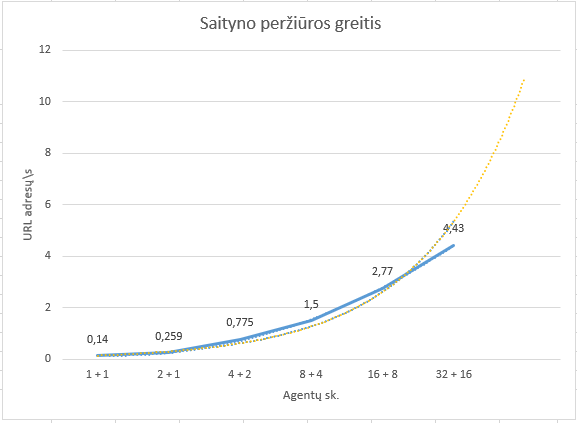
\includegraphics[scale=1]{img/saityno_peržiūros_greitis.png}
\caption{Saityno peržiūros greitis didinant agentų skaičių}
\label{fig:crawling_speed}
\end{figure}

\ref{fig:crawling_speed} diagramoje aiškiau matomas artimas eksponentiniui augimo greitis, nubrėžta trendo linija parodo, kad kitoje iteracijoje numatomas vidutinis peržiūros greitis siektų beveik 12 puslapių per sekundę.

\subsubsubsection{Javascript atvaizdavimo funkcinės metrikos}

\ref{tab:js_crawling_metrics} lentelėje matomi eksperimento statistikos duomenys, kurie pasiekti vykdant Javascript atvaizdavimą, t.y. nustačius indikaciją, jog puslapis reikalauja dinaminio, klientinės pusės atvaizdavimo (prototipo realizacijoje identifikavus, jog naudojamas klientinis karkasas).
% Table generated by Excel2LaTeX from sheet 'Sheet1'
\begin{table}[htbp]
  \centering
  \caption{Javascript agentų peržiūros funkcinės metrikos}
    \begin{tabular}{|c|c|c|c|c|}
    \toprule
    \textbf{Agentai} & \multicolumn{1}{p{7em}|}{\textbf{ Peržiūrėta URL adresų (JS)}} & \multicolumn{1}{p{7.61em}|}{\textbf{ Peržiūrėta URL adresų (JS), proc.}} & \multicolumn{1}{p{8.11em}|}{\textbf{Rasta URL adresų (JS)}} & \multicolumn{1}{p{6.78em}|}{\textbf{Rasta URL adresų (JS), proc.}} \\
    \midrule
    1 + 1 & 1     & 0,20\% & 20    & 0,79\% \\
    \midrule
    \textcolor{red}{2 + 1} & \textcolor{red}{1}     & \textcolor{red}{0,11\%} & \textcolor{red}{4}     & \textcolor{red}{0,06\%} \\
    \midrule
    4 + 2 & 246   & 8,81\% & 2147  & 7,12\% \\
    \midrule
    \textcolor{red}{8 + 4} & \textcolor{red}{213}   & \textcolor{red}{3,93\%} & \textcolor{red}{870}   & \textcolor{red}{0,77\%} \\
    \midrule
    16 + 8 & 1614  & 16,14\% & 10500 & 16,16\% \\
    \midrule
    32 + 12 & 5458  & 34,22\% & 47016 & 11,22\% \\
    \bottomrule
    \end{tabular}%
  \label{tab:js_crawling_metrics}%
\end{table}%


Raudonai pažymėtos eilutės demonstruoja iteracijas, kurių metu agentai visą skirtą eksperimentui laiką peržiūrinėjo ribotą kiekį vardų serverių, neturinčių klientinio atvaizdavimo ir turinčių didelį kiekį puslapių, dėl to demonstruoti netendencingi rodikliai (nėra augimo). Trečio ir penkto stulpelių kombinacija demonstruoja realizuoto modernių žiniatinklio programų žvalgymo, panaudojant „Chromium“ tvarkyklę ir jos naudojamą Javacript V8 variklį, naudą:
\begin{itemize}
    \item Pasitelkiant „Chromium“ tvarkyklę vidutiniškai panaudojant JS variklį pakartotinai peržiūrėta tik ~ 10,53\% puslapių -- tai leido sutaupyti daug procesoriaus ir operatyviosios atminties, taip pat tinklo resursų (tiek puslapių gavo klientinio atvaizdavimo poreikio indikaciją)
    \item Javascript atvaizdavimo metu rasta vidutiniškai 6,02\% visų žvalgymo iteracijos metu aptiktų URL adresų. Šie adresai nebūtų aptikti naudojant vieną iš tradicinių literatūroje aprašomų peržiūros robotų (pvz. \cite{HeritrixArchitecture} ar \cite{Mercator}, t.y. be „Chromium“ tvarkyklės pagalbos, todėl roboto URL duomenų bazė papildyta šiomis URL nuorodomis
\end{itemize}
\subsubsection{Bendrų peržiūros roboto komponentų apkrovos}

Šiame punkte aiškinamasi, ar kuris nors bendrasis peržiūros komponentas nelemia „butelio kaklelio“ efekto -- neartėjama prie veikimo limito ribos.

\subsubsubsection{„Service Bus“ eilių infrastruktūra}

\ref{fig:sb_užklausos} diagramoje pavaizduoti „Service Bus“ eilių stebėjimo duomenys (agentų peržiūros, kūrimo, atvaizdavimo eilės). Į užklausas įsiskaičiuoja ir eilių valdymo operacijos -- eilių agentams kūrimas, naikinimas. Jau minėta, jog „Service Bus“ bazinio paketo paslauga suteukia 1000 kreditų per sekundę, kuriuos išnaudojus, visos viršijančios užklausos atmetamos (mėlynas stulpelis rodo jų skaičių), kiekviena operacija verta 1 arba 10 kreditų, priklausomai nuo to, ar ji apibrėžia siuntimo/gavimo veiksmą, ar eilės valdymo veiksmą \cite{ServiceBusThrottlingOverview}. 
\input{chapters/figures/service_bus_užklausos}

\textbf{Kaip pastebima, sistemai dirbant 32 aktyvių agentų režimu, pradeda atsirasti atmetamų užklausų, kas rodo, jog su realizuota architektūra galimai artėjama prie „Basic“ plano siūlomų 1000 operacijų kreditų per sekundę ribos.} Norint išplėsti sistemą toliau, tektų naudoti „Premium“ planą, kuris leidžia pasitelkti dedikuotus resursus pagal reikalingą galingumo poreikį.

\pagebreak

\subsubsubsection{„Azure NoSQL Table Storage“ URL repozitorija}

\ref{fig:e2e_latency_table_storage} diagrama rodo, jog URL repozitorijos komponentas, kuris realizuotas panaudojant „Azure Table Storage“ talpinimo infrastruktūrą, išlaiko gana pastovų uždelsimą net žymiai didinat tranzakcijų skaičių per valandą (kiekviena operacija su lentelės esybe skaitoma kaip tranzakcija). Pavyzdžiui, tranzakcijų skaičiui siekiant 18400, uželsimo rodiklis buvo užfiksuotas 12,04s, o tranzakcijų skaičiui išaugus iki 209570 (daugiau nei dešimt kartų), fiksuotas labai panašus uždelsimas -- 12,13 ms. Šie tyrimo rezultatai stipriai koreliuoja su \cite{MercedCloudBasedWebCrawler} mokslininkų darytu eksperimentu, kurio metu irgi testuotas „Azure Table Storage“ E2E\footnote{End-to-End -- metrika, rodanti visą laiką, kiek truko užlausos kreipimasis, atsakymo išsiuntimas} uždelsimas. Pastebėtina, kad pastarieji savo tyrime gavo, jog 238479 tranzakcijos per valandą sugeneravo vidutinišką 8,78ms uždelsimo laiką, o rašto darbo autoriaus tyrimo metu panašiam tranzakcijų skaičiui gauta kiek didesnė nei 10ms reikšmė. Prastesnis rodiklis gali būti sietinas su priimtais skirtingais architektūros realizaciniais sprendimais, tačiau bendras rezultatas rodo, jog šis komponentas neriboja sistemos darbo augant agentų skaičiui.
\input{chapters/figures/azure_table_storage_uždelsimas}

\subsubsubsection{SQL agentų registro duomenų bazė}

Šio tyrimo metu buvo pasirinkta stebėti SQL duomenų bazės apkrovą, nes būtent ja remiasi agentų naikinimo logika. Agentų registre ant 
\begin{figure}[h]
\hspace{-1cm}
\centering
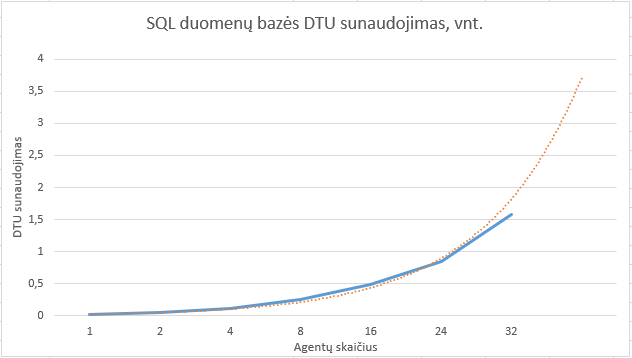
\includegraphics[scale=1]{img/sql_dtu_sunaudojimas.png}
\caption{Agentų registro SQL duombazės DTU sunaudojimas}
\label{fig:dtu_usage}
\end{figure}

